% Standalone source. Compile twice with pdflatex stage3_defog_report_draft.tex.
% Every figure is vector artwork built from the measurements embedded below.
% Data root on DTU HPC: /work3/s234818/mosaic/runs/
% Sweep: stage3-protenix-defog-lr60-3seeds-20261112a/lf-retry1/campaign/runs
% For fragmented seed 17 use both arms of projection-kkt-retry-20261117a.
% Comparison: 20261118-defog-vs-structural-repair-01,
% 20261118-structural-repair-no-projection-01, 20261119-defog-vs-repair-seeds71-101.
% Charts use raw states.jsonl.gz and summary.json. Each trajectory covers updates 0--500.
\documentclass[11pt,a4paper]{article}
\usepackage[T1]{fontenc}
\usepackage{mathpazo}
\usepackage[scaled=0.94]{helvet}
\usepackage[a4paper,left=20mm,right=20mm,top=17mm,bottom=20mm,footskip=10mm]{geometry}
\usepackage{tikz,booktabs,array,fancyhdr}
\usetikzlibrary{shapes.geometric}
\usepackage{hyperref}
\definecolor{ink}{HTML}{192F38}
\definecolor{muted}{HTML}{465C66}
\definecolor{rulegray}{HTML}{D3DCDE}
\definecolor{guide}{HTML}{006B65}
\definecolor{base}{HTML}{526879}
\definecolor{violetTen}{HTML}{704492}
\definecolor{repair}{HTML}{995019}
\definecolor{fragOK}{HTML}{82ACC6}
\definecolor{connFail}{HTML}{D59548}
\definecolor{fragFail}{HTML}{596475}
\definecolor{papergray}{HTML}{F2F5F4}
\hypersetup{colorlinks=true,urlcolor=guide,linkcolor=guide,filecolor=guide,runcolor=guide,pdftitle={Custom repair, DeFoG and projection for relaxed molecular graphs},pdfsubject={Stage 3 draft report and matched Protenix experiments}}
\pagestyle{fancy}\fancyhf{}
\renewcommand{\headrulewidth}{0pt}
\renewcommand{\footrulewidth}{0.35pt}
\fancyfoot[L]{\sffamily\footnotesize\color{muted}Mosaic\enspace/\enspace Stage 3 research draft}
\fancyfoot[R]{\sffamily\footnotesize\color{muted}\thepage\enspace/\enspace\pageref*{stage3verdict}}
\setlength{\parindent}{0pt}
\setlength{\parskip}{5pt}
\setlength{\tabcolsep}{5pt}
\color{ink}
\raggedbottom
\newcommand{\topic}[1]{{\sffamily\bfseries\small\color{guide}#1\par}\vspace{2pt}}
\newcommand{\heading}[1]{{\raggedright\fontsize{25}{28}\selectfont #1\par}\vspace{4pt}}
\newcommand{\subhead}[1]{\par\vspace{4pt}{\sffamily\bfseries\fontsize{12}{14}\selectfont #1\par}\vspace{-2pt}}
\newcommand{\ftitle}[2]{\par\vspace{5pt}{\sffamily\bfseries\fontsize{12}{14}\selectfont\textcolor{guide}{Figure #1}\quad #2\par}\vspace{-3pt}}
\newcommand{\fignote}[1]{\par\vspace{-1pt}{\small\color{muted}#1\par}}
\newcommand{\footlink}[2]{\href{#1}{#2}}
\tikzset{every node/.style={font=\sffamily\fontsize{8.6}{10}\selectfont,text=ink,inner sep=0pt},
  guidecurve/.style={draw=guide,line width=1.45pt,line join=round},
  repaircurve/.style={draw=repair,line width=1.15pt,dash pattern=on 3pt off 1.9pt,line join=round}}
\newcommand{\diamondmark}[2]{\node[diamond,fill=guide,minimum width=5.6pt,minimum height=5.6pt] at (#1,#2) {};}
\newcommand{\scorepair}[5]{%
  \node[anchor=east] at (2.25,#4) {#1};
  \draw[draw=rulegray,line width=2pt] ({2.8+42*(#2-.20)},#4) -- ({2.8+42*(#3-.20)},#4);
  \draw[draw=base,fill=white,line width=1pt] ({2.8+42*(#2-.20)},#4) circle[radius=2.5pt];
  \diamondmark{{2.8+42*(#3-.20)}}{#4}
  \node[anchor=east,text=guide] at (16.62,#4) {#5};}
\newcommand{\heatpanel}[4]{%
  \foreach \v [count=\j from 0] in {#2} {
    \pgfmathtruncatemacro{\pct}{4*\v}
    \fill[guide!\pct!papergray] ({#1+.271*\j},#3-.153) rectangle ({#1+.271*(\j+1)-.010},#3+.153);
  }
  \ifnum#4=1 \diamondmark{{#1+6.02}}{#3}
  \else \draw[muted,line width=.65pt] ({#1+5.96},#3)--({#1+6.08},#3);\fi}
\newcommand{\heatrow}[6]{%
  \node[anchor=east] at (2.65,#2) {#1};
  \heatpanel{3.00}{#3}{#2}{#5}\heatpanel{10.06}{#4}{#2}{#6}}
\newcommand{\scorepanel}[2]{%
  \node[font=\sffamily\bfseries\small,anchor=west] at (0,5.17) {Seed #1};
  \foreach \q in {0.2,0.3,0.4,0.5} {
    \draw[rulegray,line width=.35pt] (0,{9.2*\q-.16}) -- (4.55,{9.2*\q-.16});
    \ifnum#2=1 \node[anchor=east,text=muted] at (-.12,{9.2*\q-.16}) {\q};\fi}
  \foreach \u in {0,250,500} {\node[text=muted] at ({.0091*\u},1.29) {\u};}
}
\begin{document}
\topic{Molecular design\enspace/\enspace Stage 3\hfill 25 November 2026}
\heading{How do we tell an invalid molecule which bonds to change?}
Protenix can give a promising pocket-contact score to a graph that falls apart when we pick its most likely bonds. A yes/no validity test tells us that the graph failed. For optimization we also need a direction. We built the custom repair loss so we could specify which parts of the molecule a repair may change, how much an edit costs, and how strongly the proposed repair competes with pocket contact.

\subhead{What makes one repair closer than another?}
Each atom and bond has a row of probabilities. Picking the largest entry in every row gives the \emph{hard graph} (the argmax). If that graph fails, we keep its occupied slots, elements and formal charges fixed while searching for a connected, chemically valid arrangement of bonds. Each changed bond costs one, plus the log ratio of the probability of the old choice to that of the proposed choice. The matched runs gave this confidence penalty unit weight. A near tie is cheap to reverse. Overturning a confident decision costs more.

\subhead{One repair, worked through}
Imagine two fragments and two possible single bonds that could join them. Suppose either bridge alone gives a valid molecule and leaves every other bond unchanged.

\begin{center}\small\sffamily
\begin{tabular*}{.93\linewidth}{@{\extracolsep{\fill}}lrrr@{}}
\toprule
Possible bridge & $p(\mathrm{no\ bond})$ & $p(\mathrm{single})$ & Cost of the edit\\
\midrule
A\quad Nearly tied & 0.52 & 0.46 & $1+\log(0.52/0.46)=1.12$\\
B\quad Strongly favors no bond & 0.90 & 0.08 & $1+\log(0.90/0.08)=3.42$\\
\bottomrule
\end{tabular*}\end{center}
\fignote{Illustrative probabilities. The other three bond categories share the remaining 0.02 in each row.}

Both repairs take one edit. If the search finds both, it selects A. In a real graph the structural search constructs candidate backbones, trims or downgrades excess bonds, and retains the lowest-cost verified candidate it finds. Verification checks connectivity, RDKit sanitization and conversion back into the graph schema. The bounded search can miss a cheaper repair or exhaust its budget. If it finds no complete target, the fallback can use partial edits and penalties for excess valence and disconnected components.

\subhead{How a discrete repair produces a gradient}
Call the verified target $g^\star$. For this update we hold it fixed and minimize the average negative log probability of its choices, alongside the Protenix objective.
\[
  L(p)=-C_{\rm Protenix}(p)+\lambda_{\rm repair}
    \underbrace{\left[-\frac{1}{350}\sum_{r=1}^{350}\log p_r(g^\star_r)\right]}_{\rm repair\ loss\ for\ a\ complete\ target}.
\]
Here $p_r(g^\star_r)$ is the probability that row $r$ assigns to the target's choice. The 350 rows cover 25 elements, 25 fixed neutral charges and 300 unordered atom pairs. Increasing the probability of a single bond at A lowers the loss. The hard graph gains that bridge only when the single bond wins its row. The gradient flows through the probabilities. Search and chemistry checks run outside differentiation. We read the graph again at the next update. An already valid graph receives zero repair loss, so Protenix can move it again. \footlink{https://github.com/NikolajHJ/mosaic/blob/bcef814cdb07ed056a47747f47f458e59d6d97e6/src/mosaic/small_molecule/chemistry/structural.py}{Repair search} and \footlink{https://github.com/NikolajHJ/mosaic/blob/bcef814cdb07ed056a47747f47f458e59d6d97e6/src/mosaic/small_molecule/chemistry/loss.py}{loss implementation.}

\newpage
\topic{Stage 3\enspace/\enspace Custom validity loss}
\heading{What did tuning the repair change?}
In an early sparse-start run at repair weight 1, the search found a valid target at all 30,001 recorded states. The optimizer's own argmax never became valid and connected. Late in the run, fluorine still had two bonds and the proposed repair required three bond edits. The median repair gradient norm on bonds was about 6\% of the Protenix bond gradient norm over the final 5,000 updates. Averaging over the full target can dilute the signal on a few decisive bonds. This observation motivated trying stronger guidance. \footlink{https://github.com/NikolajHJ/mosaic/blob/bcef814cdb07ed056a47747f47f458e59d6d97e6/experiments/brd4-jq1/protenix-random-chem/runs/20261102-results-interpretation-01/README.md}{Trajectory analysis.}

\subhead{Which settings we varied}
The early runs updated logits at learning rate 0.3. We tried constant repair weights 1 and 10, delayed guidance, a chemistry-first period, and an adaptive weight based on the repair and contact gradient norms. We compared a bounded search over individual edits with one that first constructs a connected backbone. We also varied the starting graph, softmax temperature and added gradient-scaled noise. One 50,000-update protocol held the weight at 1 through update 20,000, raised it geometrically to 30 by update 30,000, and cooled the softmax from 0.7 to 0.4 over the run. Because this protocol changed several settings together, it cannot isolate the effect of cooling. \footlink{https://github.com/NikolajHJ/mosaic/blob/bcef814cdb07ed056a47747f47f458e59d6d97e6/experiments/brd4-jq1/protenix-random-chem/runs/20261031-chemistry-strategies-01/README.md}{Weight and temperature trials} and \footlink{https://github.com/NikolajHJ/mosaic/blob/bcef814cdb07ed056a47747f47f458e59d6d97e6/experiments/brd4-jq1/protenix-random-chem/runs/20261103-sparse-annealed-seeds-01/README.md}{annealing protocol.}

In Stage 3 we compared two repair weights on three matched five-fragment starts. We updated probabilities directly for 500 steps at learning rate 60, with unit Protenix weight, temperature 1 and projection off. Both arms allowed up to six structural candidates and 1,024 bond operations per candidate, followed by the same fallback search if needed. GPU models differed between arms.

\begin{center}\small\sffamily
\begin{tabular*}{.94\linewidth}{@{\extracolsep{\fill}}lrr@{}}
\toprule
Seeds 17, 23 and 42 & Repair weight 1 & Repair weight 10\\
\midrule
Valid, connected raw states (of 1,503) & 174 & 819\\
Runs ending valid and connected (of 3) & 1 & 3\\
Distinct valid molecules within each seed & 63, 54, 53 & 14, 10, 13\\
Mean best valid hard Protenix contact & 0.352 & 0.288\\
\bottomrule
\end{tabular*}\end{center}
Stronger repair kept more states valid but visited fewer distinct valid molecules and lowered the best contact on each seed. The counts include initialization and repeated visits. Each score is the best over one trajectory before averaging across seeds.

\subhead{Three ways to guide the same relaxed graph}
\textbf{Custom repair} chooses a specific verified graph when it can find one. Cross-entropy gives the optimizer a direction toward that graph. We can inspect the proposed edits and set their cost. Bond changes that improve pocket contact can still compete with those edits.

\textbf{DeFoG} supplies a soft target for each atom and bond from a model trained on molecules. We minimize squared distance to those predictions. A learned preference can distinguish two arrangements that both satisfy our rules, and still guide a graph after it becomes valid. Its most likely choices can also combine into disconnected fragments.

\textbf{Connected projection} acts after the gradient step. It redistributes bond probabilities to respect valence limits, attempts to bridge components and reapplies the valence rule. This can complement either loss. We evaluate the resulting hard graph to see whether the bridge survived and the molecule sanitizes.

\newpage
\topic{Stage 3\enspace/\enspace Choosing the DeFoG target}
\heading{Why stop after one DeFoG query?}
We first used DeFoG as a generator. Every five updates in the Boltz/DBMol run, we drew four candidate graphs from the decoder. For each supported candidate we started DeFoG at model time $t\approx0.8$ and sampled the remaining 447 transitions to an output molecule. We used the first eligible output as a hard target and optimized the VAE latent variable to make the decoder assign that graph higher probability. The next refresh could give the optimizer a different destination.

That happened at \textbf{all 99 successive refreshes} of the 500-update run. At 81 of those 99, even the decoder's own most likely graph was unchanged between refreshes. Sampling candidates and continuing the flow could both contribute. We kept the input fixed in a new experiment to isolate variation in the continuation itself.

\subhead{Same molecule in, how different were the targets?}
We gave the same checkpoint each of five fixed graphs at the same time. For each graph we drew eight full continuations and repeated the one-query prediction eight times. The plot counts differing atom or bond labels between two outputs with the atom slots aligned.

\begin{center}
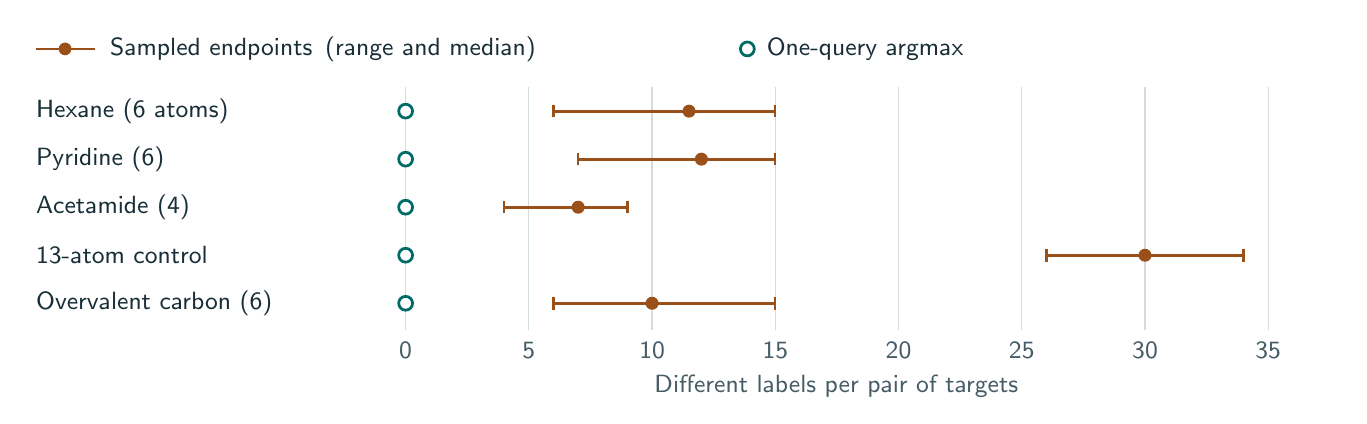
\begin{tikzpicture}[x=1cm,y=1cm]
\path[use as bounding box] (0,0) rectangle (16.65,4.68);
\draw[repair,line width=1pt] (0.1,4.41)--(0.85,4.41);
\fill[repair] (0.475,4.41) circle (2.3pt);
\node[anchor=west] at (1.04,4.41) {Sampled endpoints\enspace (range and median)};
\node[draw=guide,fill=white,line width=1pt,circle,minimum size=5pt] at (9.14,4.41) {};
\node[anchor=west] at (9.38,4.41) {One-query argmax};
\foreach \v in {0,5,10,15,20,25,30,35}{
  \draw[rulegray,line width=.45pt] ({4.8+.313*\v},.84)--({4.8+.313*\v},3.93);
  \node[text=muted] at ({4.8+.313*\v},.58) {\v};}
\foreach \name/\y/\lo/\midv/\hi in {Hexane (6 atoms)/3.62/6/11.5/15,Pyridine (6)/3.01/7/12/15,Acetamide (4)/2.40/4/7/9,13-atom control/1.79/26/30/34,Overvalent carbon (6)/1.18/6/10/15}{
  \node[anchor=west] at (.1,\y) {\name};
  \node[draw=guide,fill=white,line width=1pt,circle,minimum size=5pt] at (4.8,\y) {};
  \draw[repair,line width=1.1pt] ({4.8+.313*\lo},\y)--({4.8+.313*\hi},\y);
  \foreach \endv in {\lo,\hi} \draw[repair,line width=.8pt] ({4.8+.313*\endv},\y-.08)--({4.8+.313*\endv},\y+.08);
  \fill[repair] ({4.8+.313*\midv},\y) circle (2.35pt);}
\node[text=muted] at (10.27,.12) {Different labels per pair of targets};
\end{tikzpicture}
\end{center}
\fignote{Eight repeats give 28 overlapping pairs per control. All 140 sampled pairs differed (median 11 labels). All repeated one-query probability arrays were identical, including before taking their argmax. Larger graphs have more labels that can change.}

\subhead{What the first call gives the optimizer}
The denoiser already predicts the probability of each \emph{clean} atom and bond category before the sampler draws its next state. Stage 3 uses that prediction directly. For example, if both single and double bonds are plausible, the loss can preserve that uncertainty. We compare the current graph probabilities with the predicted probabilities, hold the prediction fixed for one update, and query again on the next graph. In the reported Protenix runs we use squared error in this shared graph representation. This requires neither a hidden-layer embedding nor a sampled first diffusion step.

We gained repeatability and reduced the cost from 447 denoiser calls per continuation to one per target. Chemical repair is a different outcome. Here \textbf{39/40 sampled endpoints} were valid and connected, while the one-query argmax qualified on \textbf{3/5 inputs}. A small input change can still flip a hard auxiliary feature. In the earlier pyridine test, moving 0.0002 probability mass across a tie changed one output row by 0.499 in total variation.

The first 1,000-update Protenix pilot kept the same valid carbon chain at every step. The later BRD4 runs tested whether the one-query loss added to projection could discover better molecules. Because the earlier Boltz run used a different scorer and optimizer, these runs cannot isolate the effect of switching teachers on the best contact score. \footlink{run:../experiments/learned-prior/protenix-defog-composition-30000/target-repeatability-20261125.md}{Experiment and sources.}

\newpage
\topic{Stage 3\enspace/\enspace DeFoG guidance}
\heading{DeFoG guidance on relaxed graphs}
At the selected weight of 0.5, adding DeFoG to connected projection improved the best valid contact score in all nine matched runs on BRD4. A better candidate could appear hundreds of updates before the final graph fragmented. We therefore evaluated both the best molecule visited and the molecule present at the end.

\subhead{A learned prior on the graph itself}
We optimized 25 atom positions directly as probabilities over six elements and five bond categories per atom pair. These Protenix experiments used no VAE encoder, decoder or latent variable. Frozen Protenix-Tiny supplied the pocket contact objective. At each update, one query to the frozen GuacaMol DeFoG model predicted clean atom and bond distributions. Its transformer read relaxed probabilities, with the current argmax supplying auxiliary features that required a discrete graph. We held the prediction fixed for one gradient update and refreshed it on the next. \footlink{https://proceedings.mlr.press/v267/qin25d.html}{Qin et al., ICML 2025.}

The loss combined negative Protenix contact with the weighted squared distance to the teacher, averaged separately over atoms and atom pairs. After the update we restored probability rows to the simplex. Connected projection also applied valence limits and attempted to bridge separate components.

\subhead{What counted as a molecule}
We chose the most likely atom and bond category at initialization and after each of 500 updates. A hard graph qualified if it passed RDKit sanitization and all 25 atoms formed one connected component. We rescored each qualifying graph with the same Protenix pocket and model key. The three seeds, crossed with three starts, give nine matched comparisons on one pocket. Contact is a model score on the discrete graph.

\ftitle{1}{DeFoG raised the best valid hard score in all nine pairs}
\begin{center}
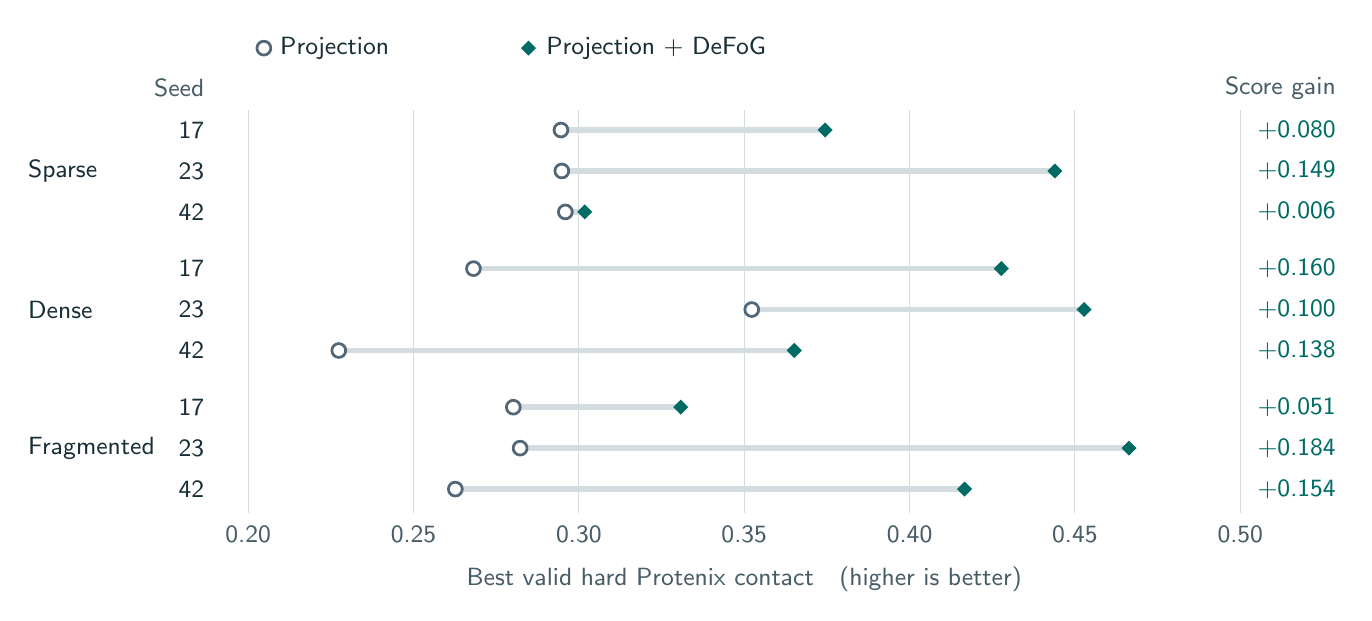
\begin{tikzpicture}[x=1cm,y=1cm]
\path[use as bounding box] (0,1.12) rectangle (16.72,8.30);
\draw[base,fill=white,line width=1pt] (3.0,8.04) circle[radius=2.5pt]; \node[anchor=west] at (3.20,8.04) {Projection};
\diamondmark{6.36}{8.04}\node[anchor=west] at (6.58,8.04) {Projection + DeFoG};
\node[anchor=east,text=muted] at (16.62,7.53) {Score gain};
\node[anchor=east,text=muted] at (2.25,7.53) {Seed};
\foreach \x/\lab in {.20/0.20,.25/0.25,.30/0.30,.35/0.35,.40/0.40,.45/0.45,.50/0.50} {
  \draw[rulegray,line width=.35pt] ({2.8+42*(\x-.20)},2.14)--({2.8+42*(\x-.20)},7.26);
  \node[text=muted] at ({2.8+42*(\x-.20)},1.87) {\lab};}
\node[anchor=west] at (0,6.48) {Sparse};\node[anchor=west] at (0,4.72) {Dense};\node[anchor=west] at (0,2.96) {Fragmented};
\scorepair{17}{0.2945808}{0.3744837}{7.00}{+0.080}
\scorepair{23}{0.2948430}{0.4439042}{6.48}{+0.149}
\scorepair{42}{0.2959213}{0.3017696}{5.96}{+0.006}
\scorepair{17}{0.2681347}{0.4277522}{5.24}{+0.160}
\scorepair{23}{0.3522849}{0.4527794}{4.72}{+0.100}
\scorepair{42}{0.2274060}{0.3651230}{4.20}{+0.138}
\scorepair{17}{0.2801797}{0.3308045}{3.48}{+0.051}
\scorepair{23}{0.2822214}{0.4663707}{2.96}{+0.184}
\scorepair{42}{0.2626559}{0.4166252}{2.44}{+0.154}
\node[text=muted] at (9.1,1.30) {Best valid hard Protenix contact\quad(higher is better)};
\end{tikzpicture}
\end{center}
\fignote{Each line joins two runs with the same seed and start at learning rate 60. DeFoG weight 0.5 and teacher time 0.8 raised the mean best score from 0.284 to 0.398. We used the completed rerun pair for fragmented seed 17 because its original projection-only control stopped early.}

\newpage
\topic{Stage 3\enspace/\enspace Projection and connectivity}
\heading{When did the graph stay connected?}
At learning rate 60, projection alone visited a valid connected graph in 54 of 4,509 states (1.2\%). With the selected DeFoG weight of 0.5 and teacher time of 0.8, that rose to 2,563 states (56.8\%). The change in the final molecule was smaller. Three of nine guided runs ended valid and connected, compared with zero of nine controls.

\ftitle{2}{Valid molecules appeared in sustained stretches on some starts}
\begin{center}
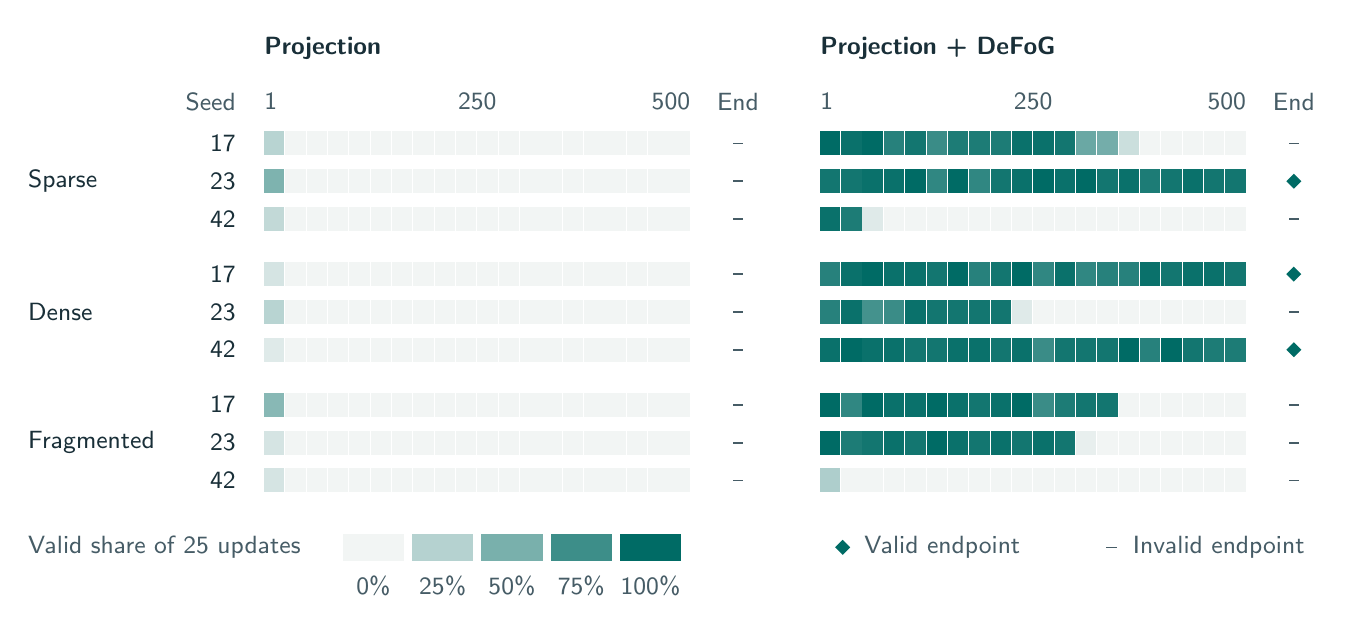
\begin{tikzpicture}[x=1cm,y=1cm]
\path[use as bounding box] (0,.43) rectangle (16.72,7.82);
\node[anchor=west,font=\sffamily\bfseries\small] at (3.00,7.56) {Projection};
\node[anchor=west,font=\sffamily\bfseries\small] at (10.06,7.56) {Projection + DeFoG};
\node[anchor=east,text=muted] at (2.65,6.88) {Seed};
\foreach \p in {3.00,10.06}{
 \node[anchor=west,text=muted] at (\p,6.88) {1};
 \node[text=muted] at ({\p+2.71},6.88) {250};
 \node[anchor=east,text=muted] at ({\p+5.42},6.88) {500};
 \node[text=muted] at ({\p+6.02},6.88) {End};}
\node[anchor=west] at (0,5.87) {Sparse};\node[anchor=west] at (0,4.21) {Dense};\node[anchor=west] at (0,2.55) {Fragmented};
\heatrow{17}{6.35}{6,0,0,0,0,0,0,0,0,0,0,0,0,0,0,0,0,0,0,0}{25,24,25,21,23,19,22,22,22,24,24,23,14,13,4,0,0,0,0,0}{0}{0}
\heatrow{23}{5.87}{12,0,0,0,0,0,0,0,0,0,0,0,0,0,0,0,0,0,0,0}{23,23,24,24,25,20,25,20,23,24,25,24,25,23,24,22,23,24,23,23}{0}{1}
\heatrow{42}{5.39}{5,0,0,0,0,0,0,0,0,0,0,0,0,0,0,0,0,0,0,0}{24,22,2,0,0,0,0,0,0,0,0,0,0,0,0,0,0,0,0,0}{0}{0}
\heatrow{17}{4.69}{3,0,0,0,0,0,0,0,0,0,0,0,0,0,0,0,0,0,0,0}{21,24,25,24,24,23,25,21,23,25,20,24,20,21,21,24,23,24,24,23}{0}{1}
\heatrow{23}{4.21}{6,0,0,0,0,0,0,0,0,0,0,0,0,0,0,0,0,0,0,0}{21,24,18,19,24,23,23,23,23,2,0,0,0,0,0,0,0,0,0,0}{0}{0}
\heatrow{42}{3.73}{2,0,0,0,0,0,0,0,0,0,0,0,0,0,0,0,0,0,0,0}{24,25,24,24,23,23,24,24,23,24,19,23,23,23,25,21,25,23,22,22}{0}{1}
\heatrow{17}{3.03}{11,0,0,0,0,0,0,0,0,0,0,0,0,0,0,0,0,0,0,0}{25,20,25,24,24,25,24,23,24,25,19,22,23,23,0,0,0,0,0,0}{0}{0}
\heatrow{23}{2.55}{3,0,0,0,0,0,0,0,0,0,0,0,0,0,0,0,0,0,0,0}{25,22,23,24,23,25,24,23,24,23,24,23,1,0,0,0,0,0,0,0}{0}{0}
\heatrow{42}{2.07}{3,0,0,0,0,0,0,0,0,0,0,0,0,0,0,0,0,0,0,0}{7,0,0,0,0,0,0,0,0,0,0,0,0,0,0,0,0,0,0,0}{0}{0}
\node[anchor=west,text=muted] at (0,1.22) {Valid share of 25 updates};
\foreach \v/\lab [count=\i from 0] in {0/0,25/25,50/50,75/75,100/100} {
 \fill[guide!\v!papergray] ({4+.88*\i},1.05) rectangle ({4.78+.88*\i},1.39);
 \node[text=muted] at ({4.39+.88*\i},.73) {\lab\%};}
\diamondmark{10.35}{1.22}\node[anchor=west,text=muted] at (10.62,1.22) {Valid endpoint};
\draw[muted] (13.70,1.22)--(13.84,1.22);\node[anchor=west,text=muted] at (14.03,1.22) {Invalid endpoint};
\end{tikzpicture}
\end{center}
\fignote{Read left to right within each method. Each cell covers 25 successive updates. The endpoint symbol records update 500 separately. The totals above include initialization, which is omitted from the grid. Adjacent observations follow the same trajectory.}

\subhead{What improved, and what remained difficult}
Guided runs visited 7--468 distinct valid molecules each. More valid observations therefore included changes of molecular identity. Yet the mean absolute difference between relaxed and hard contact, measured over all states, grew from 0.021 to 0.039. Better archived candidates did not come with closer agreement between the two scores. Weight 0.5 was selected from this sweep.

At weight 0.0625 without Stage 2 projection, DeFoG found zero new valid molecules across nine runs. The three valid observations were the initially connected sparse graphs. Adding connected projection at that weight produced a new valid identity in every run, with zero valid endpoints. Holding the initial teacher target fixed also gave a higher mean best score than refreshing it at each step (0.347 versus 0.318 at weight 0.0625 with projection). The weight-0.5 standalone comparison appears on page~\pageref{lastreportpage}.

\subhead{Why earlier runs looked more stable}
From a connected carbon chain at learning rate 0.3, weight 0.0625 plus projection retained validity for 1,998 of 2,001 observations and visited 68 distinct molecules. In a separate 10,000-update pair with the same chain and cyclic weight schedule, raising the learning rate from 0.3 to 150 reduced valid connected observations from 9,958 to 39. These runs show the importance of reporting the starting graph and update size. \footlink{https://github.com/NikolajHJ/mosaic/blob/e1b57fc2cab68e17a39c366aa3fbb8c21a0ff2a9/src/mosaic/small_molecule/Stage3/BENCHMARKS.md}{Historical benchmark tables.}

\newpage
\topic{Stage 3\enspace/\enspace Custom loss comparison}
\heading{Can either method join five fragments?}
The custom loss searches for an atom-preserving repair of the current graph. When the graph already qualifies, the repair loss falls to zero. We compared projected DeFoG at weight 0.5 with unprojected repair at weight 1 on five seeds. Three of those seeds also received unprojected repair at weight 10. All arms used the same starting graph and Protenix key within seed, LR 60, 500 updates and a 0.0001 uniform mixture. The new runs used an A100. Earlier optimization runs used other GPU models.

\ftitle{3}{How quickly did each run find its best valid molecule?}
\begin{center}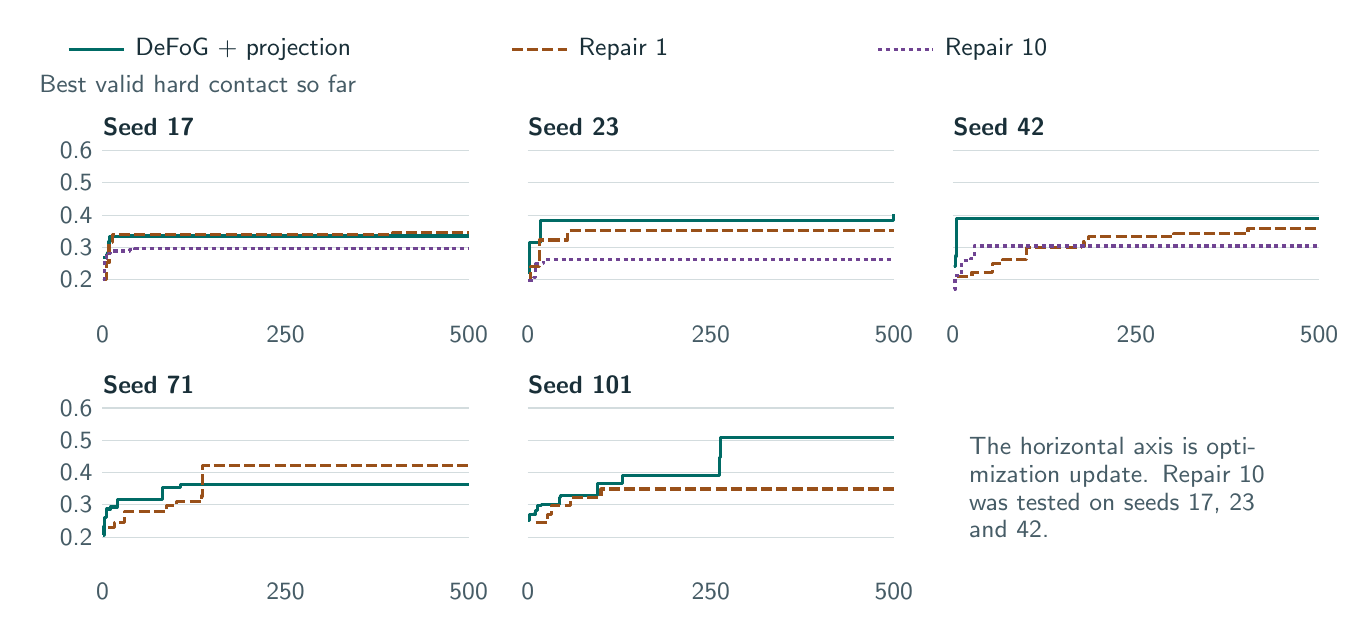
\begin{tikzpicture}[x=1cm,y=1cm]
\path[use as bounding box] (0,0) rectangle (16.70,7.40);
\draw[guide,line width=1.2pt,solid] (0.52,7.12)--(1.22,7.12);\node[anchor=west] at (1.3599999999999999,7.12) {DeFoG + projection};
\draw[repair,line width=1.2pt,dash pattern=on 4pt off 1.5pt] (6.15,7.12)--(6.8500000000000005,7.12);\node[anchor=west] at (6.99,7.12) {Repair 1};
\draw[violetTen,line width=1.2pt,dash pattern=on 1.5pt off 1.3pt] (10.8,7.12)--(11.5,7.12);\node[anchor=west] at (11.64,7.12) {Repair 10};
\node[anchor=west,text=muted] at (.14,6.69) {Best valid hard contact so far};
\begin{scope}[shift={(0.95,3.45)}]
\node[anchor=west,font=\sffamily\bfseries\small] at (0,2.69) {Seed 17};
\draw[rulegray,thin] (0,0.7500)--(4.65,0.7500);
\node[anchor=east,text=muted] at (-.12,0.7500) {0.2};
\draw[rulegray,thin] (0,1.1600)--(4.65,1.1600);
\node[anchor=east,text=muted] at (-.12,1.1600) {0.3};
\draw[rulegray,thin] (0,1.5700)--(4.65,1.5700);
\node[anchor=east,text=muted] at (-.12,1.5700) {0.4};
\draw[rulegray,thin] (0,1.9800)--(4.65,1.9800);
\node[anchor=east,text=muted] at (-.12,1.9800) {0.5};
\draw[rulegray,thin] (0,2.3900)--(4.65,2.3900);
\node[anchor=east,text=muted] at (-.12,2.3900) {0.6};
\node[text=muted] at (0,.06) {0};
\node[text=muted] at (2.3249999999999997,.06) {250};
\node[text=muted] at (4.6499999999999995,.06) {500};
\draw[guide,solid,line width=1.15pt,line join=round] (0.0093,1.0345) -| (0.0558,1.0677) -| (0.0651,1.0942) -| (0.0837,1.2366) -| (0.0930,1.2928) -| (0.3348,1.3032) -| (4.6500,1.3032);
\draw[repair,dash pattern=on 4pt off 1.5pt,line width=1.15pt,line join=round] (0.0093,0.7517) -| (0.0558,0.9640) -| (0.0837,1.2207) -| (0.1302,1.3231) -| (3.6828,1.3521) -| (4.6500,1.3521);
\draw[violetTen,dash pattern=on 1.5pt off 1.3pt,line width=1.15pt,line join=round] (0.0093,0.7517) -| (0.0279,1.0160) -| (0.0558,1.0515) -| (0.0837,1.0867) -| (0.1023,1.1132) -| (0.3441,1.1323) -| (0.4092,1.1419) -| (4.6500,1.1419);
\end{scope}
\begin{scope}[shift={(6.35,3.45)}]
\node[anchor=west,font=\sffamily\bfseries\small] at (0,2.69) {Seed 23};
\draw[rulegray,thin] (0,0.7500)--(4.65,0.7500);
\draw[rulegray,thin] (0,1.1600)--(4.65,1.1600);
\draw[rulegray,thin] (0,1.5700)--(4.65,1.5700);
\draw[rulegray,thin] (0,1.9800)--(4.65,1.9800);
\draw[rulegray,thin] (0,2.3900)--(4.65,2.3900);
\node[text=muted] at (0,.06) {0};
\node[text=muted] at (2.3249999999999997,.06) {250};
\node[text=muted] at (4.6499999999999995,.06) {500};
\draw[guide,solid,line width=1.15pt,line join=round] (0.0093,0.8447) -| (0.0186,1.1073) -| (0.0279,1.2190) -| (0.1674,1.4989) -| (4.6500,1.5853);
\draw[repair,dash pattern=on 4pt off 1.5pt,line width=1.15pt,line join=round] (0.0093,0.7340) -| (0.0372,0.9167) -| (0.1488,1.2524) -| (0.5022,1.3719) -| (4.6500,1.3719);
\draw[violetTen,dash pattern=on 1.5pt off 1.3pt,line width=1.15pt,line join=round] (0.0093,0.7399) -| (0.0744,0.7803) -| (0.1023,0.9525) -| (0.2046,1.0080) -| (4.6500,1.0080);
\end{scope}
\begin{scope}[shift={(11.75,3.45)}]
\node[anchor=west,font=\sffamily\bfseries\small] at (0,2.69) {Seed 42};
\draw[rulegray,thin] (0,0.7500)--(4.65,0.7500);
\draw[rulegray,thin] (0,1.1600)--(4.65,1.1600);
\draw[rulegray,thin] (0,1.5700)--(4.65,1.5700);
\draw[rulegray,thin] (0,1.9800)--(4.65,1.9800);
\draw[rulegray,thin] (0,2.3900)--(4.65,2.3900);
\node[text=muted] at (0,.06) {0};
\node[text=muted] at (2.3249999999999997,.06) {250};
\node[text=muted] at (4.6499999999999995,.06) {500};
\draw[guide,solid,line width=1.15pt,line join=round] (0.0093,0.9168) -| (0.0186,0.9205) -| (0.0372,1.0510) -| (0.0465,1.5315) -| (4.6500,1.5315);
\draw[repair,dash pattern=on 4pt off 1.5pt,line width=1.15pt,line join=round] (0.0558,0.7921) -| (0.2418,0.8446) -| (0.5022,0.9509) -| (0.5952,0.9526) -| (0.6324,1.0087) -| (0.9393,1.1565) -| (1.6368,1.1747) -| (1.6647,1.2395) -| (1.7205,1.2941) -| (2.8086,1.3313) -| (3.7479,1.4000) -| (4.6500,1.4000);
\draw[violetTen,dash pattern=on 1.5pt off 1.3pt,line width=1.15pt,line join=round] (0.0093,0.6232) -| (0.0279,0.7994) -| (0.1116,0.9894) -| (0.2232,1.0187) -| (0.2697,1.1781) -| (4.6500,1.1781);
\end{scope}
\begin{scope}[shift={(0.95,0.18)}]
\node[anchor=west,font=\sffamily\bfseries\small] at (0,2.69) {Seed 71};
\draw[rulegray,thin] (0,0.7500)--(4.65,0.7500);
\node[anchor=east,text=muted] at (-.12,0.7500) {0.2};
\draw[rulegray,thin] (0,1.1600)--(4.65,1.1600);
\node[anchor=east,text=muted] at (-.12,1.1600) {0.3};
\draw[rulegray,thin] (0,1.5700)--(4.65,1.5700);
\node[anchor=east,text=muted] at (-.12,1.5700) {0.4};
\draw[rulegray,thin] (0,1.9800)--(4.65,1.9800);
\node[anchor=east,text=muted] at (-.12,1.9800) {0.5};
\draw[rulegray,thin] (0,2.3900)--(4.65,2.3900);
\node[anchor=east,text=muted] at (-.12,2.3900) {0.6};
\node[text=muted] at (0,.06) {0};
\node[text=muted] at (2.3249999999999997,.06) {250};
\node[text=muted] at (4.6499999999999995,.06) {500};
\draw[guide,solid,line width=1.15pt,line join=round] (0.0093,0.7771) -| (0.0186,0.8888) -| (0.0279,0.9967) -| (0.0558,1.1077) -| (0.1023,1.1316) -| (0.1860,1.2315) -| (0.7626,1.3825) -| (0.9951,1.4166) -| (4.6500,1.4166);
\draw[repair,dash pattern=on 4pt off 1.5pt,line width=1.15pt,line join=round] (0.0744,0.8751) -| (0.1488,0.9337) -| (0.2790,1.0705) -| (0.8091,1.1481) -| (0.9393,1.1974) -| (1.2555,1.2729) -| (1.2741,1.6628) -| (4.6500,1.6628);
\end{scope}
\begin{scope}[shift={(6.35,0.18)}]
\node[anchor=west,font=\sffamily\bfseries\small] at (0,2.69) {Seed 101};
\draw[rulegray,thin] (0,0.7500)--(4.65,0.7500);
\draw[rulegray,thin] (0,1.1600)--(4.65,1.1600);
\draw[rulegray,thin] (0,1.5700)--(4.65,1.5700);
\draw[rulegray,thin] (0,1.9800)--(4.65,1.9800);
\draw[rulegray,thin] (0,2.3900)--(4.65,2.3900);
\node[text=muted] at (0,.06) {0};
\node[text=muted] at (2.3249999999999997,.06) {250};
\node[text=muted] at (4.6499999999999995,.06) {500};
\draw[guide,solid,line width=1.15pt,line join=round] (0.0093,0.9599) -| (0.0186,1.0422) -| (0.0744,1.0424) -| (0.0837,1.0447) -| (0.1023,1.0842) -| (0.1209,1.1525) -| (0.1767,1.1591) -| (0.4092,1.2495) -| (0.4185,1.2753) -| (0.5859,1.2767) -| (0.8835,1.4308) -| (1.2090,1.5298) -| (2.2692,1.5376) -| (2.4366,1.7614) -| (2.4459,2.0104) -| (4.6500,2.0104);
\draw[repair,dash pattern=on 4pt off 1.5pt,line width=1.15pt,line join=round] (0.1023,0.9391) -| (0.2511,1.0373) -| (0.2976,1.1519) -| (0.5487,1.2557) -| (0.9300,1.3622) -| (4.6500,1.3622);
\end{scope}
\node[anchor=west,text width=3.8cm,align=left,text=muted] at (11.95,1.56) {The horizontal axis is optimization update. Repair 10 was tested on seeds 17, 23 and 42.};
\end{tikzpicture}\end{center}
\fignote{Each curve starts at the first valid molecule and rises only when the optimizer finds a better one. A level stretch can include fragmented molecules. All panels use the same axes.}

\begin{center}\small\sffamily
\begin{tabular*}{.97\linewidth}{@{\extracolsep{\fill}}lrrr rrr@{}}
\toprule
&\multicolumn{3}{c}{Best valid hard contact}&\multicolumn{3}{c}{Valid states / final components}\\
\cmidrule(lr){2-4}\cmidrule(l){5-7}
Seed & DeFoG & Repair 1 & Repair 10 & DeFoG & Repair 1 & Repair 10\\
\midrule
17 & 0.335 & 0.347 & 0.296 & 47\,/\,4 & 63\,/\,1 & 328\,/\,1\\
23 & 0.404 & 0.352 & 0.263 & 440\,/\,1 & 57\,/\,2 & 249\,/\,1\\
42 & 0.391 & 0.359 & 0.304 & 38\,/\,4 & 54\,/\,3 & 242\,/\,1\\
71 & 0.363 & 0.423 & -- & 101\,/\,6 & 57\,/\,1 & --\\
101 & 0.507 & 0.349 & -- & 243\,/\,6 & 60\,/\,3 & --\\
\bottomrule\end{tabular*}\end{center}
Repair 10 found a valid connected molecule on 3 of the three starts and ended valid on 3. On these same starts, mean best contact was 0.376 for projected DeFoG, 0.352 for repair 1 and 0.288 for repair 10. Weight 10 visited 14, 10, 13 distinct valid identities on seeds 17, 23 and 42, respectively, versus 63, 54 and 53 at weight 1. Its best molecules appeared by update 44. Across all five seeds, DeFoG led repair 1 on best valid contact in three pairs (mean 0.400 versus 0.366). Both found valid molecules on all five seeds. Seed 101 accounted for most of the mean advantage. Without it, the means were 0.373 and 0.370.

With projection held on for both losses on the three original seeds, DeFoG led repair 1 in two pairs. Across the five main pairs, a post hoc check capped each run at its first 20 distinct valid molecules. Mean best contact was 0.345 for projected DeFoG and 0.359 for repair 1. The full 500-update comparison also rewards methods that discover more candidates.

\newpage
\topic{Stage 3\enspace/\enspace Fresh-key evaluation}
\heading{Do the selected molecules keep their scores?}
Before rescoring, we fixed the five highest-scoring distinct valid molecules from each of the 16 runs in the structural-repair comparison, preserving their ordered atom and bond tensors. We rescored every selected graph on one A100 with five common fresh Protenix keys (7001--7005) and replayed its original key. The primary comparison follows each run's original winner. The secondary comparison averages the full shortlist. Selection used only optimization-key scores.

\ftitle{4}{How far did the best molecule lead its shortlist?}
\begin{center}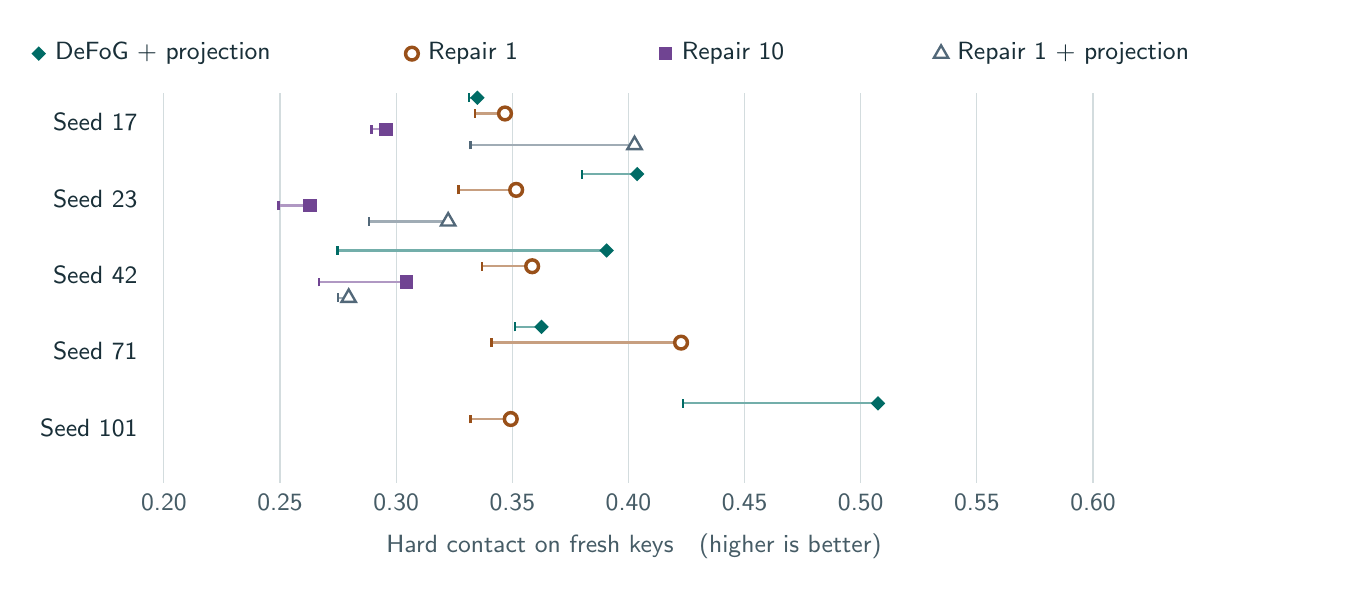
\begin{tikzpicture}[x=1cm,y=1cm]
\path[use as bounding box] (0,0) rectangle (16.72,6.8);
\node[diamond,fill=guide,minimum size=5.4pt] at (0.14,6.47) {};\node[anchor=west] at (0.34,6.47) {DeFoG + projection};
\draw[repair,line width=1.25pt,fill=white] (4.88,6.47) circle[radius=2.3pt];\node[anchor=west] at (5.08,6.47) {Repair 1};
\node[rectangle,fill=violetTen,minimum size=4.8pt] at (8.1,6.47) {};\node[anchor=west] at (8.299999999999999,6.47) {Repair 10};
\node[regular polygon,regular polygon sides=3,draw=base,fill=white,line width=.85pt,minimum size=6pt] at (11.6,6.47) {};\node[anchor=west] at (11.799999999999999,6.47) {Repair 1 + projection};
\draw[rulegray,thin] (1.730,1.02)--(1.730,5.97);\node[text=muted] at (1.730,.77) {0.20};
\draw[rulegray,thin] (3.205,1.02)--(3.205,5.97);\node[text=muted] at (3.205,.77) {0.25};
\draw[rulegray,thin] (4.680,1.02)--(4.680,5.97);\node[text=muted] at (4.680,.77) {0.30};
\draw[rulegray,thin] (6.155,1.02)--(6.155,5.97);\node[text=muted] at (6.155,.77) {0.35};
\draw[rulegray,thin] (7.630,1.02)--(7.630,5.97);\node[text=muted] at (7.630,.77) {0.40};
\draw[rulegray,thin] (9.105,1.02)--(9.105,5.97);\node[text=muted] at (9.105,.77) {0.45};
\draw[rulegray,thin] (10.580,1.02)--(10.580,5.97);\node[text=muted] at (10.580,.77) {0.50};
\draw[rulegray,thin] (12.055,1.02)--(12.055,5.97);\node[text=muted] at (12.055,.77) {0.55};
\draw[rulegray,thin] (13.530,1.02)--(13.530,5.97);\node[text=muted] at (13.530,.77) {0.60};
\node[anchor=east] at (1.4,5.6) {Seed 17};
\draw[guide!55!white,line width=.83pt] (5.603,5.91)--(5.710,5.91);\draw[guide,line width=.9pt] (5.603,5.853)--(5.603,5.967);\node[diamond,fill=guide,minimum size=5.4pt] at (5.710,5.91) {};
\draw[repair!55!white,line width=.83pt] (5.681,5.71)--(6.062,5.71);\draw[repair,line width=.9pt] (5.681,5.653)--(5.681,5.767);\draw[repair,line width=1.25pt,fill=white] (6.062,5.71) circle[radius=2.3pt];
\draw[violetTen!55!white,line width=.83pt] (4.366,5.51)--(4.549,5.51);\draw[violetTen,line width=.9pt] (4.366,5.453)--(4.366,5.567);\node[rectangle,fill=violetTen,minimum size=4.8pt] at (4.549,5.51) {};
\draw[base!55!white,line width=.83pt] (5.621,5.31)--(7.707,5.31);\draw[base,line width=.9pt] (5.621,5.253)--(5.621,5.367);\node[regular polygon,regular polygon sides=3,draw=base,fill=white,line width=.85pt,minimum size=6pt] at (7.707,5.31) {};
\node[anchor=east] at (1.4,4.63) {Seed 23};
\draw[guide!55!white,line width=.83pt] (7.040,4.94)--(7.740,4.94);\draw[guide,line width=.9pt] (7.040,4.883)--(7.040,4.997);\node[diamond,fill=guide,minimum size=5.4pt] at (7.740,4.94) {};
\draw[repair!55!white,line width=.83pt] (5.472,4.74)--(6.204,4.74);\draw[repair,line width=.9pt] (5.472,4.683)--(5.472,4.797);\draw[repair,line width=1.25pt,fill=white] (6.204,4.74) circle[radius=2.3pt];
\draw[violetTen!55!white,line width=.83pt] (3.186,4.54)--(3.586,4.54);\draw[violetTen,line width=.9pt] (3.186,4.483)--(3.186,4.597);\node[rectangle,fill=violetTen,minimum size=4.8pt] at (3.586,4.54) {};
\draw[base!55!white,line width=.83pt] (4.335,4.34)--(5.340,4.34);\draw[base,line width=.9pt] (4.335,4.283)--(4.335,4.397);\node[regular polygon,regular polygon sides=3,draw=base,fill=white,line width=.85pt,minimum size=6pt] at (5.340,4.34) {};
\node[anchor=east] at (1.4,3.6599999999999997) {Seed 42};
\draw[guide!55!white,line width=.83pt] (3.936,3.97)--(7.353,3.97);\draw[guide,line width=.9pt] (3.936,3.913)--(3.936,4.027);\node[diamond,fill=guide,minimum size=5.4pt] at (7.353,3.97) {};
\draw[repair!55!white,line width=.83pt] (5.769,3.77)--(6.407,3.77);\draw[repair,line width=.9pt] (5.769,3.713)--(5.769,3.827);\draw[repair,line width=1.25pt,fill=white] (6.407,3.77) circle[radius=2.3pt];
\draw[violetTen!55!white,line width=.83pt] (3.703,3.57)--(4.810,3.57);\draw[violetTen,line width=.9pt] (3.703,3.513)--(3.703,3.627);\node[rectangle,fill=violetTen,minimum size=4.8pt] at (4.810,3.57) {};
\draw[base!55!white,line width=.83pt] (3.939,3.37)--(4.077,3.37);\draw[base,line width=.9pt] (3.939,3.313)--(3.939,3.427);\node[regular polygon,regular polygon sides=3,draw=base,fill=white,line width=.85pt,minimum size=6pt] at (4.077,3.37) {};
\node[anchor=east] at (1.4,2.6899999999999995) {Seed 71};
\draw[guide!55!white,line width=.83pt] (6.191,3.00)--(6.526,3.00);\draw[guide,line width=.9pt] (6.191,2.943)--(6.191,3.057);\node[diamond,fill=guide,minimum size=5.4pt] at (6.526,3.00) {};
\draw[repair!55!white,line width=.83pt] (5.892,2.80)--(8.298,2.80);\draw[repair,line width=.9pt] (5.892,2.743)--(5.892,2.857);\draw[repair,line width=1.25pt,fill=white] (8.298,2.80) circle[radius=2.3pt];
\node[anchor=east] at (1.4,1.7199999999999998) {Seed 101};
\draw[guide!55!white,line width=.83pt] (8.321,2.03)--(10.799,2.03);\draw[guide,line width=.9pt] (8.321,1.973)--(8.321,2.087);\node[diamond,fill=guide,minimum size=5.4pt] at (10.799,2.03) {};
\draw[repair!55!white,line width=.83pt] (5.625,1.83)--(6.135,1.83);\draw[repair,line width=.9pt] (5.625,1.773)--(5.625,1.887);\draw[repair,line width=1.25pt,fill=white] (6.135,1.83) circle[radius=2.3pt];
\node[text=muted] at (7.7,.22) {Hard contact on fresh keys\quad(higher is better)};
\end{tikzpicture}\end{center}
\fignote{The symbol marks the original winner and the vertical tick marks the mean of its top five molecules. Both use fresh-key scores. A long line means the winner scored well above the rest of its shortlist.}

\begin{center}\small\sffamily
\begin{tabular*}{.97\linewidth}{@{\extracolsep{\fill}}lcrrr@{}}
\toprule
& & \multicolumn{2}{c}{Original winner} & All shortlisted molecules\\
\cmidrule(lr){3-4}\cmidrule(l){5-5}
Method & Seeds & Archived & Fresh mean & Fresh mean\\
\midrule
DeFoG + projection & 5 & 0.400 & 0.400 & 0.352\\
Repair 1 & 5 & 0.366 & 0.366 & 0.334\\
\addlinespace
DeFoG + projection & 3 & 0.376 & 0.376 & 0.329\\
Repair 1 & 3 & 0.352 & 0.352 & 0.333\\
Repair 10 & 3 & 0.288 & 0.288 & 0.269\\
Repair 1 + projection & 3 & 0.335 & 0.335 & 0.298\\
\bottomrule\end{tabular*}\end{center}
Across 80 candidates from 16 runs, the largest within-graph range across the five fresh keys was zero. The largest absolute difference between an archived score and its original-key replay on the A100 was less than one millionth. Every fresh-key evaluation exactly matched its original-key replay on the same A100. Changing the key supplied no independent score variation for these graphs in this inference configuration.

Projected DeFoG gave the higher mean best score on the five-seed comparison. On the three shared starts, repair 10 retained connectivity at the endpoint every time, with lower best scores on all three. Fresh keys preserved these rankings, but evaluating one fixed pocket and model leaves performance on other targets open. \footlink{https://github.com/NikolajHJ/mosaic/blob/e1b57fc2cab68e17a39c366aa3fbb8c21a0ff2a9/docs/defog_status_2026-11-19/agent_reference.md}{Stage 3 methods.}
\newpage
\topic{Stage 3\enspace/\enspace Standalone DeFoG}
\heading{Does DeFoG need projection at weight 0.5?}
\phantomsection\label{lastreportpage}
We removed the Stage 2 valence and connectivity operators from the selected DeFoG setup. Each of three runs started with the same five fragments and Protenix key as its projected counterpart. Both kept the probability simplex update, the uniform mixture of 0.0001, teacher weight 0.5, teacher time 0.8, learning rate 60 and a 500-update budget. Initial graph tensors, model weights and pocket context matched. The new trajectories ran on an A100. The projected comparisons used other GPU models.

\ftitle{5}{Which hard graphs did the two methods visit?}
\begin{center}
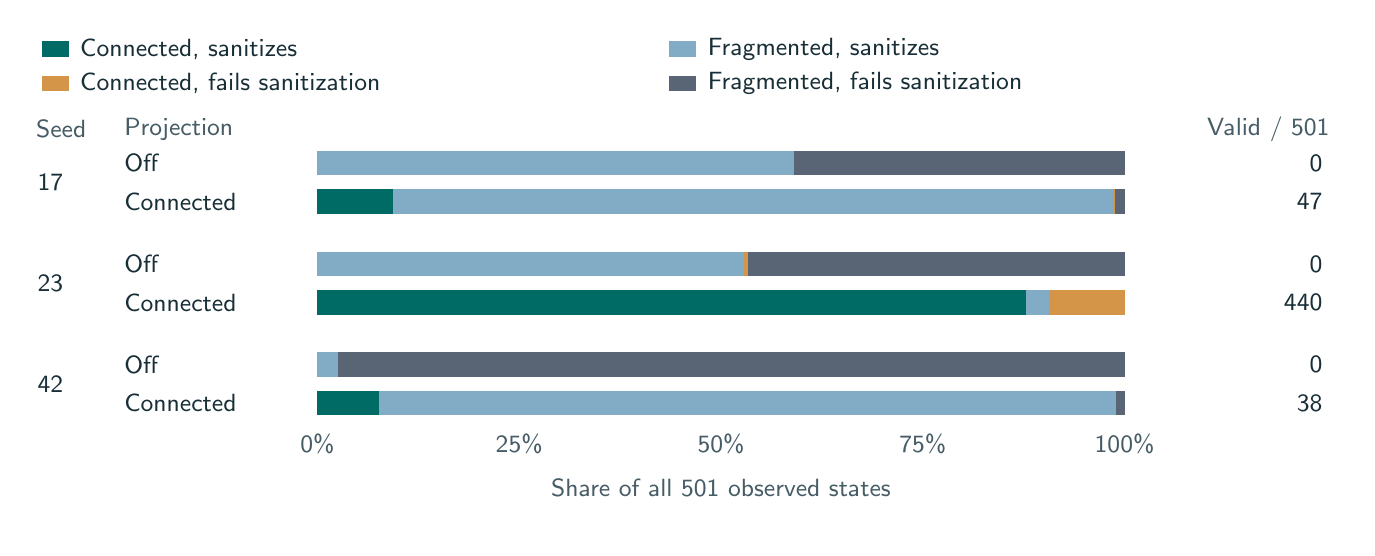
\begin{tikzpicture}[x=1cm,y=1cm]
\path[use as bounding box] (0,0) rectangle (16.75,6.35);
\fill[guide] (0.18,5.98) rectangle (0.52,6.18);\node[anchor=west] at (0.6599999999999999,6.08) {Connected, sanitizes};
\fill[fragOK] (8.15,5.98) rectangle (8.49,6.18);\node[anchor=west] at (8.63,6.08) {Fragmented, sanitizes};
\fill[connFail] (0.18,5.54) rectangle (0.52,5.739999999999999);\node[anchor=west] at (0.6599999999999999,5.64) {Connected, fails sanitization};
\fill[fragFail] (8.15,5.54) rectangle (8.49,5.739999999999999);\node[anchor=west] at (8.63,5.64) {Fragmented, fails sanitization};
\node[anchor=west,text=muted] at (.1,5.06) {Seed};\node[anchor=west,text=muted] at (1.22,5.06) {Projection};\node[anchor=east,text=muted] at (16.54,5.06) {Valid / 501};
\node[anchor=west] at (.12,4.385) {17};
\node[anchor=west] at (1.22,4.63) {Off};
\fill[fragOK] (3.6800,4.475) rectangle (9.7359,4.785);
\fill[fragFail] (9.7359,4.475) rectangle (13.9300,4.785);
\node[anchor=east] at (16.45,4.63) {0};
\node[anchor=west] at (1.22,4.14) {Connected};
\fill[guide] (3.6800,3.985) rectangle (4.6416,4.295);
\fill[fragOK] (4.6416,3.985) rectangle (13.7868,4.295);
\fill[connFail] (13.7868,3.985) rectangle (13.8072,4.295);
\fill[fragFail] (13.8072,3.985) rectangle (13.9300,4.295);
\node[anchor=east] at (16.45,4.14) {47};
\node[anchor=west] at (.12,3.105) {23};
\node[anchor=west] at (1.22,3.35) {Off};
\fill[fragOK] (3.6800,3.195) rectangle (9.1017,3.505);
\fill[connFail] (9.1017,3.195) rectangle (9.1426,3.505);
\fill[fragFail] (9.1426,3.195) rectangle (13.9300,3.505);
\node[anchor=east] at (16.45,3.35) {0};
\node[anchor=west] at (1.22,2.8600000000000003) {Connected};
\fill[guide] (3.6800,2.705) rectangle (12.6820,3.015);
\fill[fragOK] (12.6820,2.705) rectangle (12.9684,3.015);
\fill[connFail] (12.9684,2.705) rectangle (13.9300,3.015);
\node[anchor=east] at (16.45,2.8600000000000003) {440};
\node[anchor=west] at (.12,1.8249999999999997) {42};
\node[anchor=west] at (1.22,2.07) {Off};
\fill[fragOK] (3.6800,1.915) rectangle (3.9460,2.225);
\fill[fragFail] (3.9460,1.915) rectangle (13.9300,2.225);
\node[anchor=east] at (16.45,2.07) {0};
\node[anchor=west] at (1.22,1.5799999999999996) {Connected};
\fill[guide] (3.6800,1.425) rectangle (4.4574,1.735);
\fill[fragOK] (4.4574,1.425) rectangle (13.8277,1.735);
\fill[fragFail] (13.8277,1.425) rectangle (13.9300,1.735);
\node[anchor=east] at (16.45,1.5799999999999996) {38};
\node[text=muted] at (3.68,1.07) {0\%};
\node[text=muted] at (6.2425,1.07) {25\%};
\node[text=muted] at (8.805,1.07) {50\%};
\node[text=muted] at (11.3675,1.07) {75\%};
\node[text=muted] at (13.93,1.07) {100\%};
\node[text=muted] at (8.805,.50) {Share of all 501 observed states};
\end{tikzpicture}
\end{center}
\fignote{Each bar contains the initial graph and 500 updated graphs. A qualifying molecule is both connected and RDKit-sanitizable (dark green). The right column gives the exact number of qualifying states. Very narrow bands can be difficult to see.}

\begin{center}\small\sffamily
\begin{tabular*}{.97\linewidth}{@{\extracolsep{\fill}}llrrrc@{}}
\toprule
Seed & Projection & Best valid contact & Distinct valid & Final components & Final valid\\
\midrule
17 & Off & -- & 0 & 6 & No \\
17 & Connected & 0.335 & 47 & 4 & No \\
23 & Off & -- & 0 & 2 & No \\
23 & Connected & 0.404 & 440 & 1 & Yes \\
42 & Off & -- & 0 & 7 & No \\
42 & Connected & 0.391 & 36 & 4 & No \\
\bottomrule\end{tabular*}\end{center}
\fignote{A dash denotes a run with no eligible molecule for hard-contact comparison. Distinct molecules are counted by canonical SMILES within each run.}

\subhead{Finding and retaining valid molecules}
Without projection, 1,501 of 1,503 graphs were fragmented. All 574 graphs that passed sanitization had multiple components. Seed 23 briefly reached a single component twice, but both graphs failed sanitization. With connected projection, all three seeds found valid molecules, accounting for 525 of 1,503 states (34.9\%). Seed 23 also ended valid.

For this BRD4 search, DeFoG at weight 0.5 supplied useful guidance alongside connected projection. On its own it yielded no valid candidate from the three fragmented starts. Returning the best valid molecule visited preserves the benefit of the projected search. If the final iterate itself must be valid, custom repair at weight 10 achieved that outcome on all three starts, with lower best contact scores.

\newpage
\topic{Stage 3\enspace/\enspace What the learned prior can repair}
\heading{Does DeFoG point toward a valid edit?}
\phantomsection\label{stage3verdict}
We selected 12 distinct valid 25-atom molecules from the BRD4 shortlists. From each molecule we made two controlled defects. Removing one bridge split it into two sanitizable fragments. Increasing a single bond to double created a valence violation. We kept an untouched copy as a control. Every graph received one frozen DeFoG query at time 0.8.

We ranked all 1,200 possible single-bond label substitutions by how much a move toward the teacher would improve their margin over the current label. RDKit checked which edits restored validity and connectivity with all atom labels held fixed. This gives credit to any verified repair, including alternatives to restoring the original bond.

\begin{center}\small\sffamily
\begin{tabular*}{.97\linewidth}{@{\extracolsep{\fill}}lrr@{}}
\toprule
Measure & Bridge deleted & Valence violation\\
\midrule
Probability rose for the original bond label & 10/12 & 12/12\\
Median rank of the original bond label & 132 & 5\\
Median rank of the best verified repair & 28.5 & 3\\
Best verified repair ranked in the top ten & 1/12 & 12/12\\
Valid after a 25\% move toward the teacher & 0/12 & 0/12\\
Valid after a 75\% move toward the teacher & 0/12 & 2/12\\
Valid at the teacher argmax & 0/12 & 1/12\\
\bottomrule
\end{tabular*}\end{center}

A good rank means the teacher points toward a repair. The chosen label still has to overtake the current winner, and other atom and bond predictions can change at the same time. Every untouched control stayed valid after a quarter-step or half-step, and eight stayed valid after a three-quarter-step. The probe therefore gives stronger evidence for recognizing a local valence error than for repairing a cut in the graph. \footlink{run:../experiments/learned-prior/protenix-defog-composition-30000/teacher-mechanism-20261125.md}{Protocol and raw results.}

\subhead{How the results line up with the Stage 3 criteria}
\textbf{Hard validity and fragmentation.} Alongside projection, DeFoG increased valid observations from 54 to 2,563 out of 4,509. Only three of nine guided runs finished valid. The three fragmented starts without projection yielded zero valid readouts, consistent with weak connectivity guidance in the bridge probe.

\textbf{Agreement between relaxed and hard scores.} The mean absolute score gap grew from 0.021 to 0.039. Choosing the best hard molecule remains important even when the relaxed search visits more valid graphs.

\textbf{Contact score and exploration.} The selected teacher improved best valid hard contact in all nine BRD4 comparisons with projection alone. Those guided runs found 7 to 468 distinct valid molecules. The earlier 1,000-update pilot stayed on one carbon chain, so exploration depends on the optimization setup. The strongest evidence supports retrieving the best valid molecule visited with the tested projection settings. \footlink{https://github.com/NikolajHJ/mosaic/blob/2eeeba20261633cd297ff79b15b527465ead890e/docs/project_desc.pdf}{Project description, \S 6.3.}
\end{document}
